Scientists typically have to seek out the aid of software developers in order to obtain configuration files that matched their specifications. This is currently being done manually by editing large JSON files which is both fragile as well as time-consuming for both parties involved.

The NeXus Constructor is a tool written in Qt for Python which allows scientists to create, edit and visualise NeXus files and their equivalent JSON files with minimal assistance. Such files can then be used for configuring the experiment control software in order to write real-time data. The screenshot shows the main window of the NeXus Constructor and its "Add Component" dialog which allows users to add extra data in a NeXus file that describes the components that were present in an experiment. % Someone may not know what experiment control software does, what makes real-time data good, etc.

\begin{figure}
\caption{Screenshot of the NeXus Constructor}
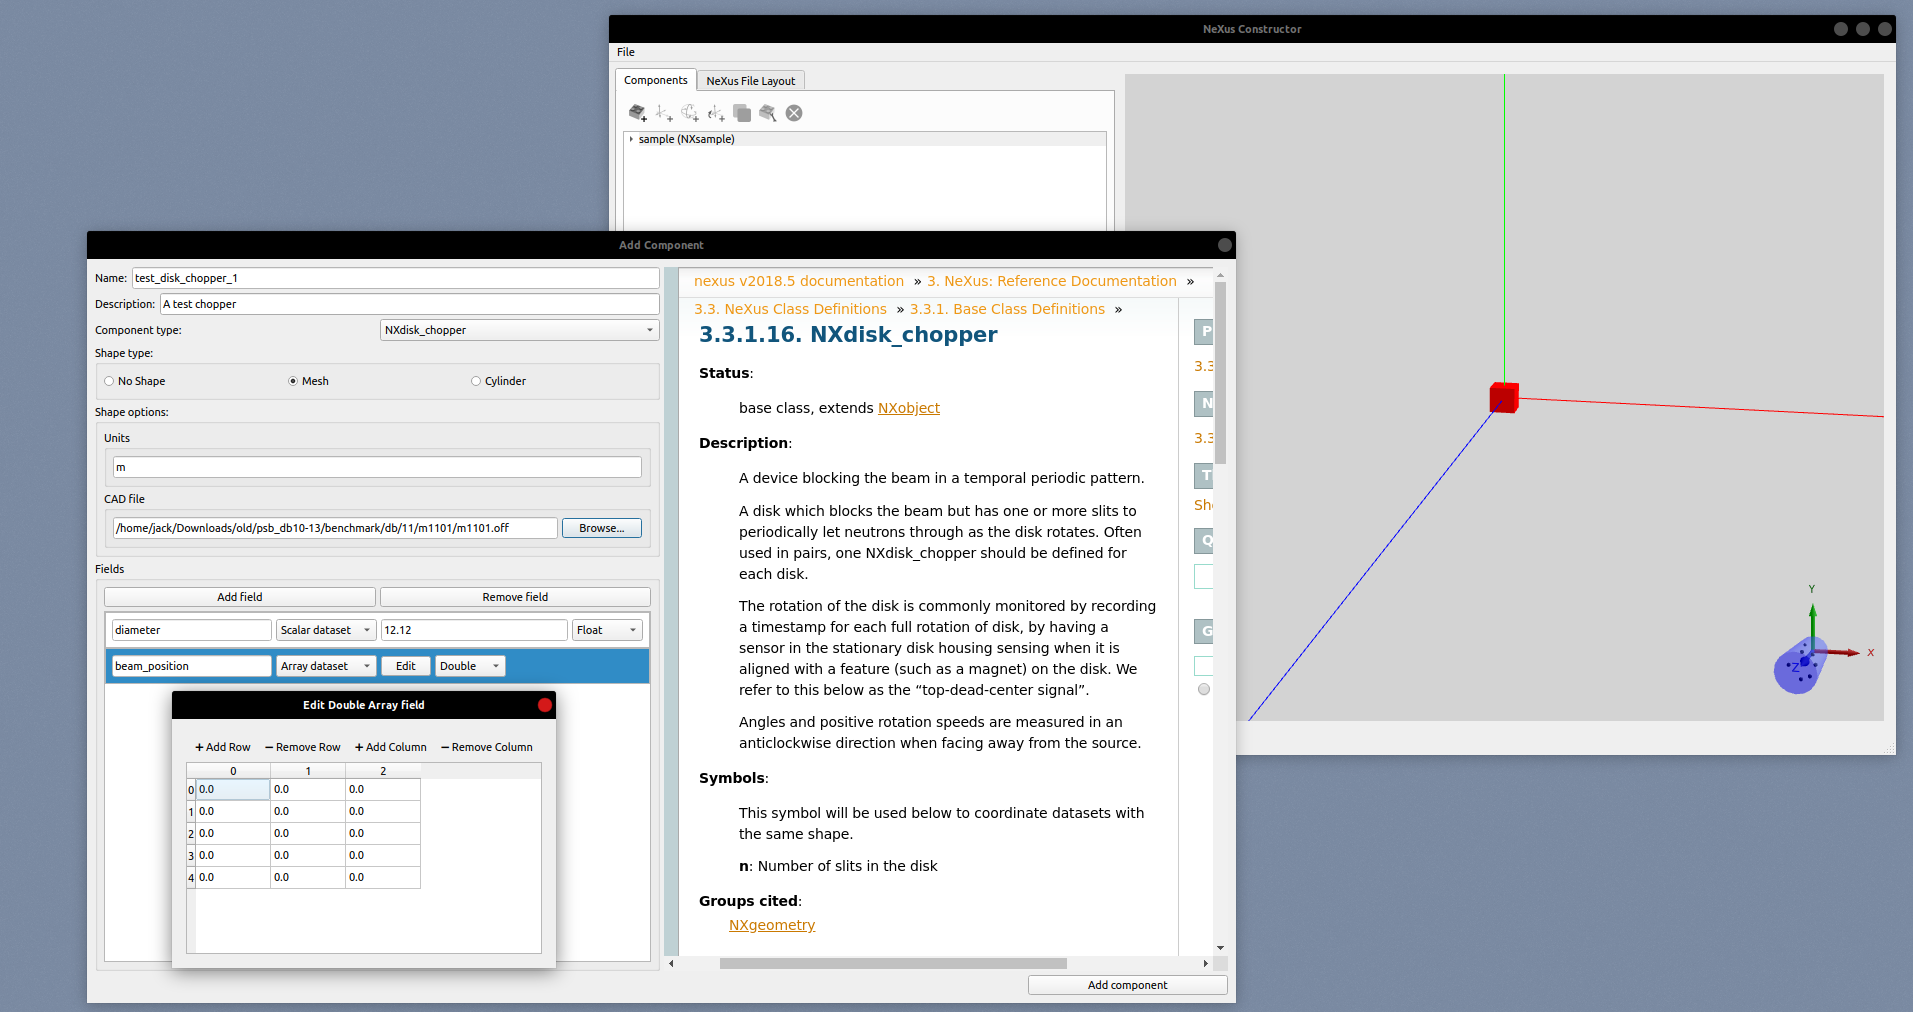
\includegraphics[width=\linewidth]{screenshot.png}
\end{figure}




